\section{Base Teórica}

La planificación es un componente fundamental del sistema operativo que se encarga de asignar tiempo de procesamiento a los diferentes hilos y procesos que se ejecutan en un sistema. En este capítulo se presentará la información necesaria para comprender la planificación a corto plazo, con un enfoque específico en el sistema operativo FreeBSD y su planificador 4BSD. Se describirán los conceptos fundamentales de procesos e hilos, incluyendo su estructura y estados, y se explicará cómo el planificador toma decisiones sobre cuál hilo o proceso debe ejecutarse en un momento dado. Además, se examinarán en detalle las operaciones de cambio de contexto, encolado, elección del procesador y remoción de hilos de la cola, que son funciones clave del planificador 4BSD. Con esta base teórica, se sentarán las bases para entender cómo funciona el planificador de FreeBSD y cómo puede ser mejorado.


\subsection{Procesos e hilos}

En sistemas operativos, los procesos son entidades aisladas que representan la ejecución de una tarea o aplicación en particular. Cada proceso cuenta con su propio espacio de direcciones, que es un área reservada de memoria virtual donde se aloja el código del programa, las variables y los recursos necesarios para su ejecución. Además, disponen de acceso a los recursos del kernel a través de llamadas a sistemas.\par

Cada proceso puede alojar uno o varios hilos de ejecución. Estos son subunidades dentro de un proceso que pueden ejecutarse de manera independiente, y comparten los recursos del mismo. Cada hilo se corresponde con un procesador virtual que cuenta con su propio contexto y un stack de ejecución que se aloja en el espacio de direcciones del proceso.\par

El kernel del sistema operativo soporta la ilusión de ejecución concurrente de múltiples procesos al repartir los recursos del sistema entre los procesadores que están listos para ejecutar.\par

\subsubsection{Estructura de los procesos}
Cada proceso en el sistema recibe un identificador único llamado identificador de proceso (PID). Los PID son el mecanismo común utilizado por las aplicaciones y el kernel para hacer referencia a los procesos. Existen dos identificadores que son de especial importancia para cada proceso: el PID del proceso en sí, y el PID del proceso padre.\par

La estructura simplificada de un proceso se puede observar en la Figura \ref{fig:process_state}. El objetivo es permitir múltiples hilos que compartan un espacio de direcciones y otros recursos.  Algunas de estas categorías son:\par

\begin{itemize}
    \item Identificación del grupo de procesos: el grupo de procesos y la sesión a la que pertenece el mismo.
    \item Credenciales de usuario: los identificadores de usuario y grupo.
    \item Gestión de memoria: la estructura que describe el espacio de direcciones virtuales utilizado por el proceso.
    \item Descriptores de archivos: una matriz de punteros que indica los archivos abiertos por el proceso e información relevante de los mismos.
    \item Vector de llamadas al sistema: estructura de datos que mapea las llamadas al sistema con las funciones correspondientes en el kernel del sistema operativo.
    \item Contabilidad de recursos: estructura que describe la utilización de los recursos del sistema..
    \item Estadísticas: estadísticas del proceso sobre su ejecución, temporizadores y profiling.
    \item Acciones de señal: la acción a tomar cuando se envía una señal a un proceso.
    \item Estructura de hilo: el contenido de la estructura de hilos del proceso.
\end{itemize}

\begin{figure}[H]
    \centering
    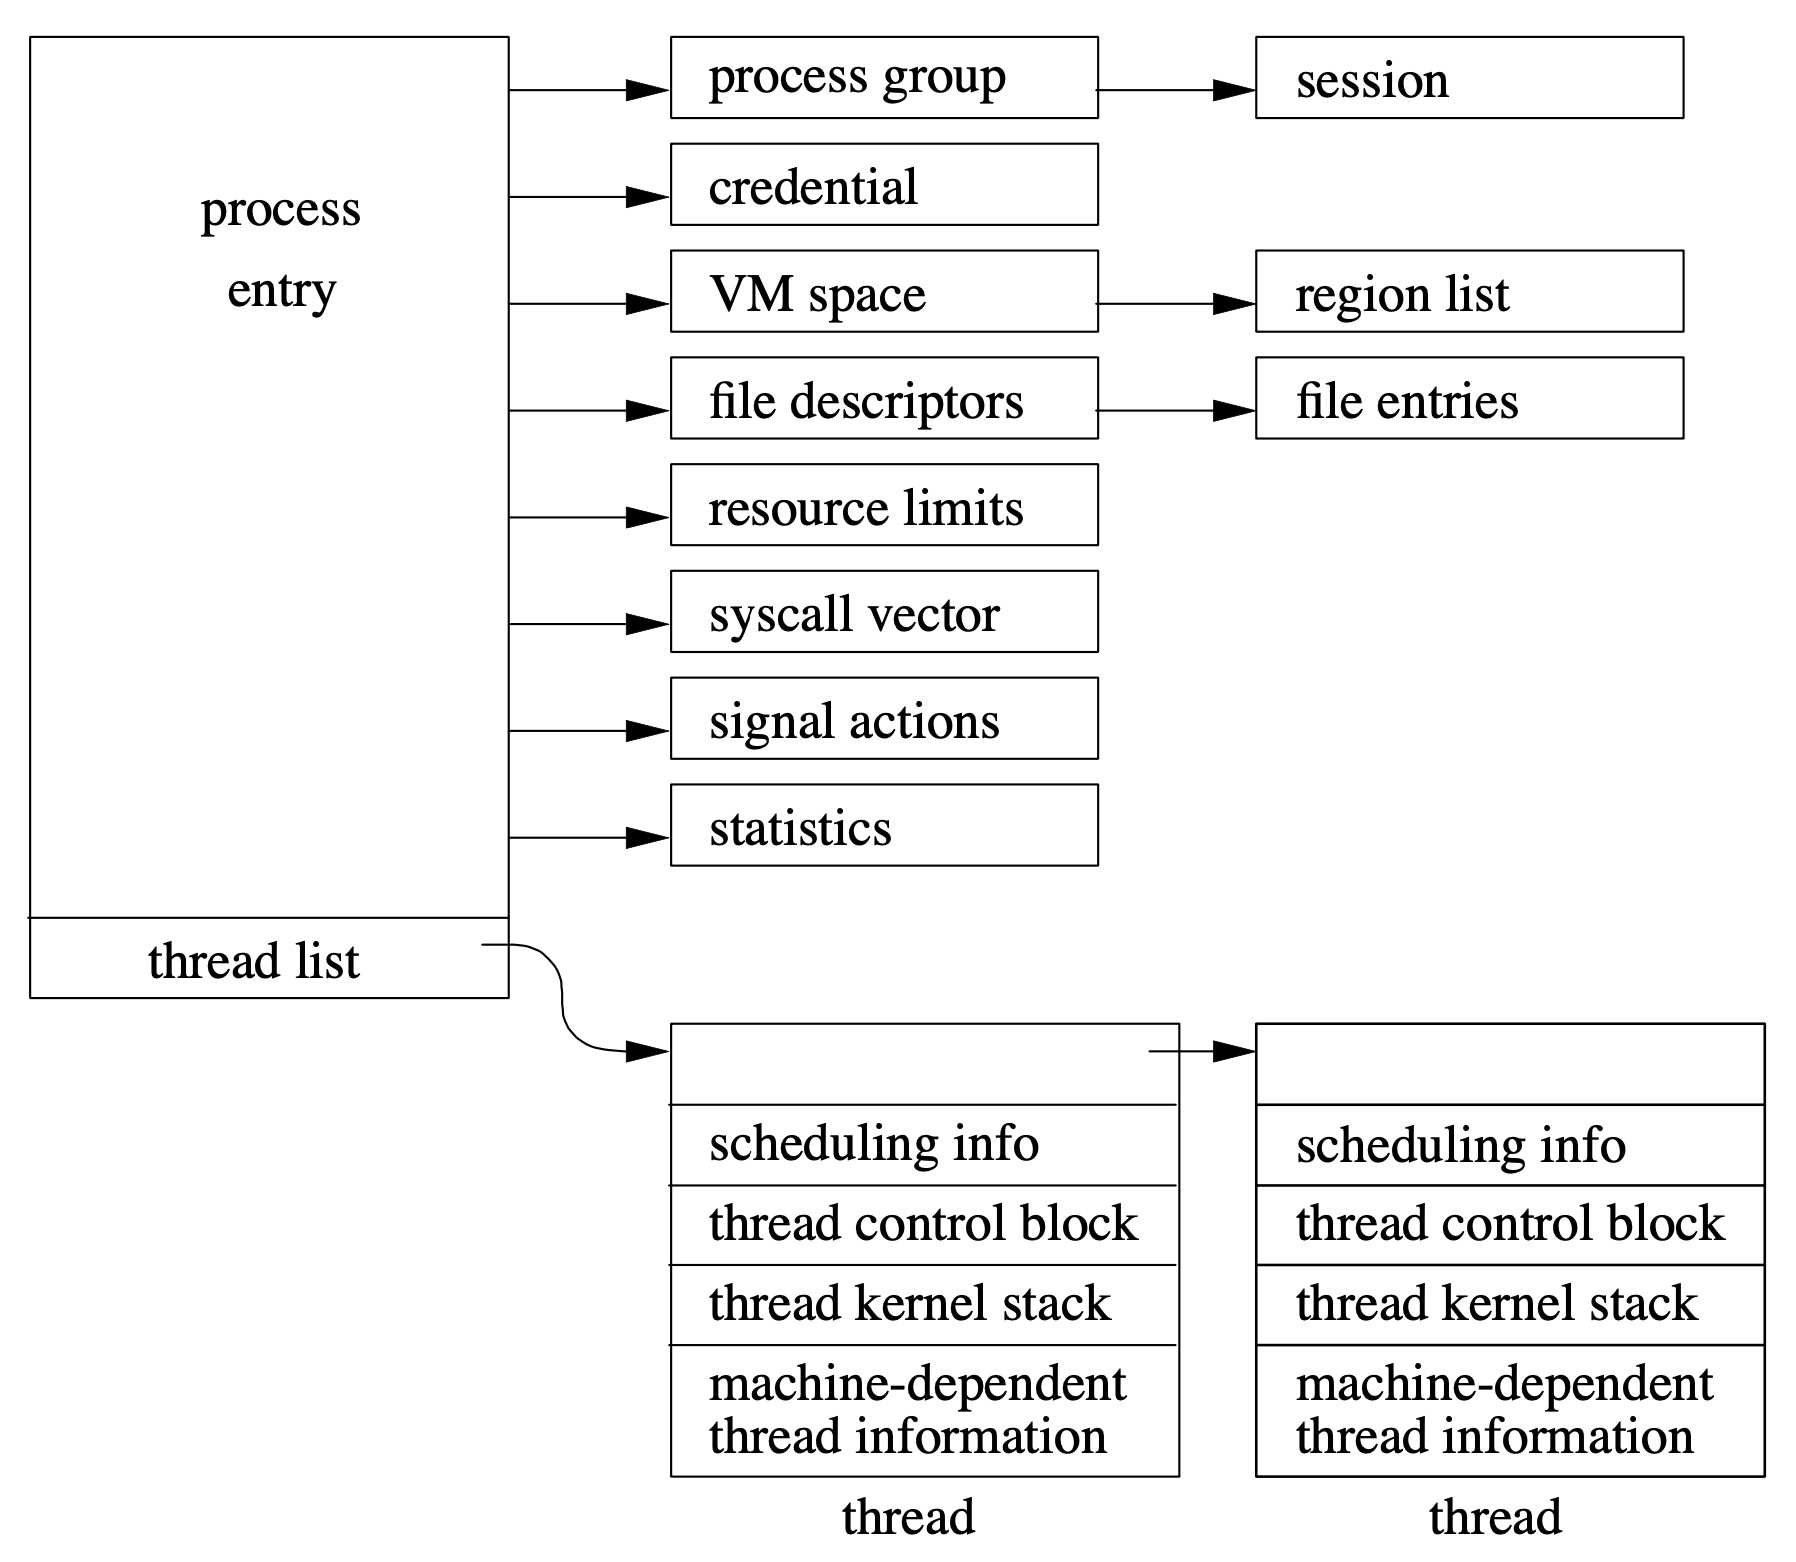
\includegraphics[width=0.6\textwidth]{images/processStructure.png}
    \caption{Estructura simplificada de un proceso.}
    \label{fig:process_state}
\end{figure}

\subsubsection{Estructura de hilos}
Un hilo, en el contexto de un proceso en un sistema operativo, es una entidad de ejecución que representa una secuencia independiente de instrucciones dentro de ese proceso. Cada hilo tiene su propio contador de programa, registros de CPU y pila de ejecución, lo que le permite ejecutar código de manera concurrente dentro del mismo proceso. Aunque los hilos comparten recursos como el espacio de direcciones y otros recursos del proceso principal, también pueden comunicarse y cooperar entre sí para llevar a cabo tareas específicas de manera más eficiente.\par

FreeBSD adopta el modelo 1:1, en el que cada hilo de usuario se corresponde con un hilo a nivel de kernel para mejorar la eficiencia de las aplicaciones.\par

La estructura de un hilo, que se muestra en la Figura \ref{fig:process_state}, solo contiene la información necesaria para ejecutarse en el kernel del sistema operativo:

\begin{itemize}
    \item Información para la planificación: se refiere a la prioridad del hilo en modo kernel y en modo usuario, la cantidad de tiempo que ha pasado suspendido y el uso reciente de la CPU. Además, se indica el estado de ejecución del hilo, banderas de estado adicionales; y si el hilo se encuentra suspendido, información sobre el canal y evento por el cual espera.
    \item TSB (thread state block): estado de ejecución del hilo en modo usuario y modo kernel. La estructura incluye registros de propósito general, punteros de pila, contador de programa, registros de gestión de memoria, entre otros.
    \item Pila del kernel: pila para usar al ejecutar en el kernel. Las pilas del kernel deben mantenerse pequeñas para evitar desperdiciar memoria física.
    \item Estado de la máquina (\textit{machine-dependent state}): se refiere a la información del hilo en relación a detalles que son específicos de la arquitectura de la CPU (registros de estado de punto flotante, información de interrupciones, información de registros de segmento de memoria, etc.).
\end{itemize}

\subsubsection{Estados de los procesos e hilos}

En FreeBSD, los procesos pueden encontrarse en uno de tres estados:

\begin{itemize}
    \item \uppercase{New}: Cuando se crea un proceso con la llamada al sistema fork.
    \item \uppercase{Normal}: El proceso pasa a este estado al asignarse suficientes recursos, permitiéndole comenzar su ejecución.
    \item \uppercase{Zombie}: Cuando un proceso ha completado su ejecución. En este estado, el proceso ha finalizado, pero aún no ha liberado todos sus recursos y no ha notificado su estado de finalización a su proceso padre.
\end{itemize}

El scheduler se encarga de planificar aquellos hilos correspondientes a procesos en estado NORMAL. Los hilos que conforman un proceso pueden encontrarse en diferentes estados:

\begin{itemize}
    \item \uppercase{inactive}: En proceso de creación y aún no han sido inicializados.
    \item \uppercase{inhibited}: Esperando por algún recurso del sistema o evento antes de poder ejecutarse.
    \item \uppercase{can\_run}: Inicializados y disponibles para ser agregados a alguna cola de ejecución.
    \item \uppercase{runq}: En la cola de ejecución, esperando su turno para ser ejecutados.
    \item \uppercase{running}: En ejecución.
\end{itemize}
